\documentclass[11pt,a4paper]{ctexart}
\usepackage[margin=18mm]{geometry}
\usepackage{graphicx}
\usepackage{xcolor}
\usepackage{booktabs}
\usepackage{array}
\usepackage{longtable}
\usepackage{tikz}
\usepackage{hyperref}
\usepackage{listings}
\usetikzlibrary{arrows.meta,positioning,calc}

\hypersetup{colorlinks=true,linkcolor=blue,urlcolor=blue}
\definecolor{bluewire}{HTML}{2563EB}
\definecolor{greenwire}{HTML}{16A34A}
\definecolor{orangewire}{HTML}{EA580C}
\definecolor{graywire}{HTML}{475569}
\definecolor{board}{HTML}{111827}
\definecolor{sensor}{HTML}{F8FAFC}

\lstset{basicstyle=\ttfamily\small,breaklines=true,frame=single,columns=fullflexible}

\title{STM32H743IIT6 测量头：AS7343 光谱 + TSL2591 强度\\接线、采样、屏幕绘图与启动图设计}
\author{stm32dev / DualLampHI}
\date{2026-07-01}

\begin{document}
\maketitle

\section{当前目标}

你现在想把“灯控制”和“测量”分离：

\begin{itemize}
  \item Arduino 继续负责两路灯的 PWM 控制；
  \item STM32H743IIT6 核心板只负责测量、显示和数据输出；
  \item AS7343 负责光谱指纹；
  \item TSL2591 负责总强度；
  \item 屏幕画图不能影响最快采样。
\end{itemize}

当前 Windows 检测结果：只看到 \texttt{COM1}，没有看到 ST-Link、USB CDC、CMSIS-DAP 或 STM32 串口。OpenOCD attach 返回：

\begin{lstlisting}
Error: open failed
\end{lstlisting}

所以目前传感器即使已经接到 STM32，我也还不能从电脑直接 flash 或读取 STM32。需要先让 ST-Link/SWD 或 USB 串口在 Windows 中出现。

\section{推荐接线}

第一版使用一条 3.3 V I2C 总线。两个传感器并联到同一组 SDA/SCL。

\begin{longtable}{>{\ttfamily}p{24mm} p{34mm} p{34mm} p{34mm}}
\toprule
STM32 丝印 & 功能 & AS7343 & TSL2591\\
\midrule
3.3 & 3.3 V 电源 & VCC / VIN & VCC / VIN\\
GND & 地 & GND & GND\\
B8 & PB8 / I2C1\_SCL & SCL & SCL\\
B9 & PB9 / I2C1\_SDA & SDA & SDA\\
不接 & 中断以后再用 & INT/GPIO 暂不接 & INT 暂不接\\
\bottomrule
\end{longtable}

注意：第一版不要把传感器同时接到 Arduino 和 STM32。I2C 总线可以挂多个从机，但不建议让 Arduino 和 STM32 同时作为 master 驱动同一组 SDA/SCL。

\section{板子照片和找针方法}

\begin{figure}[h]
\centering
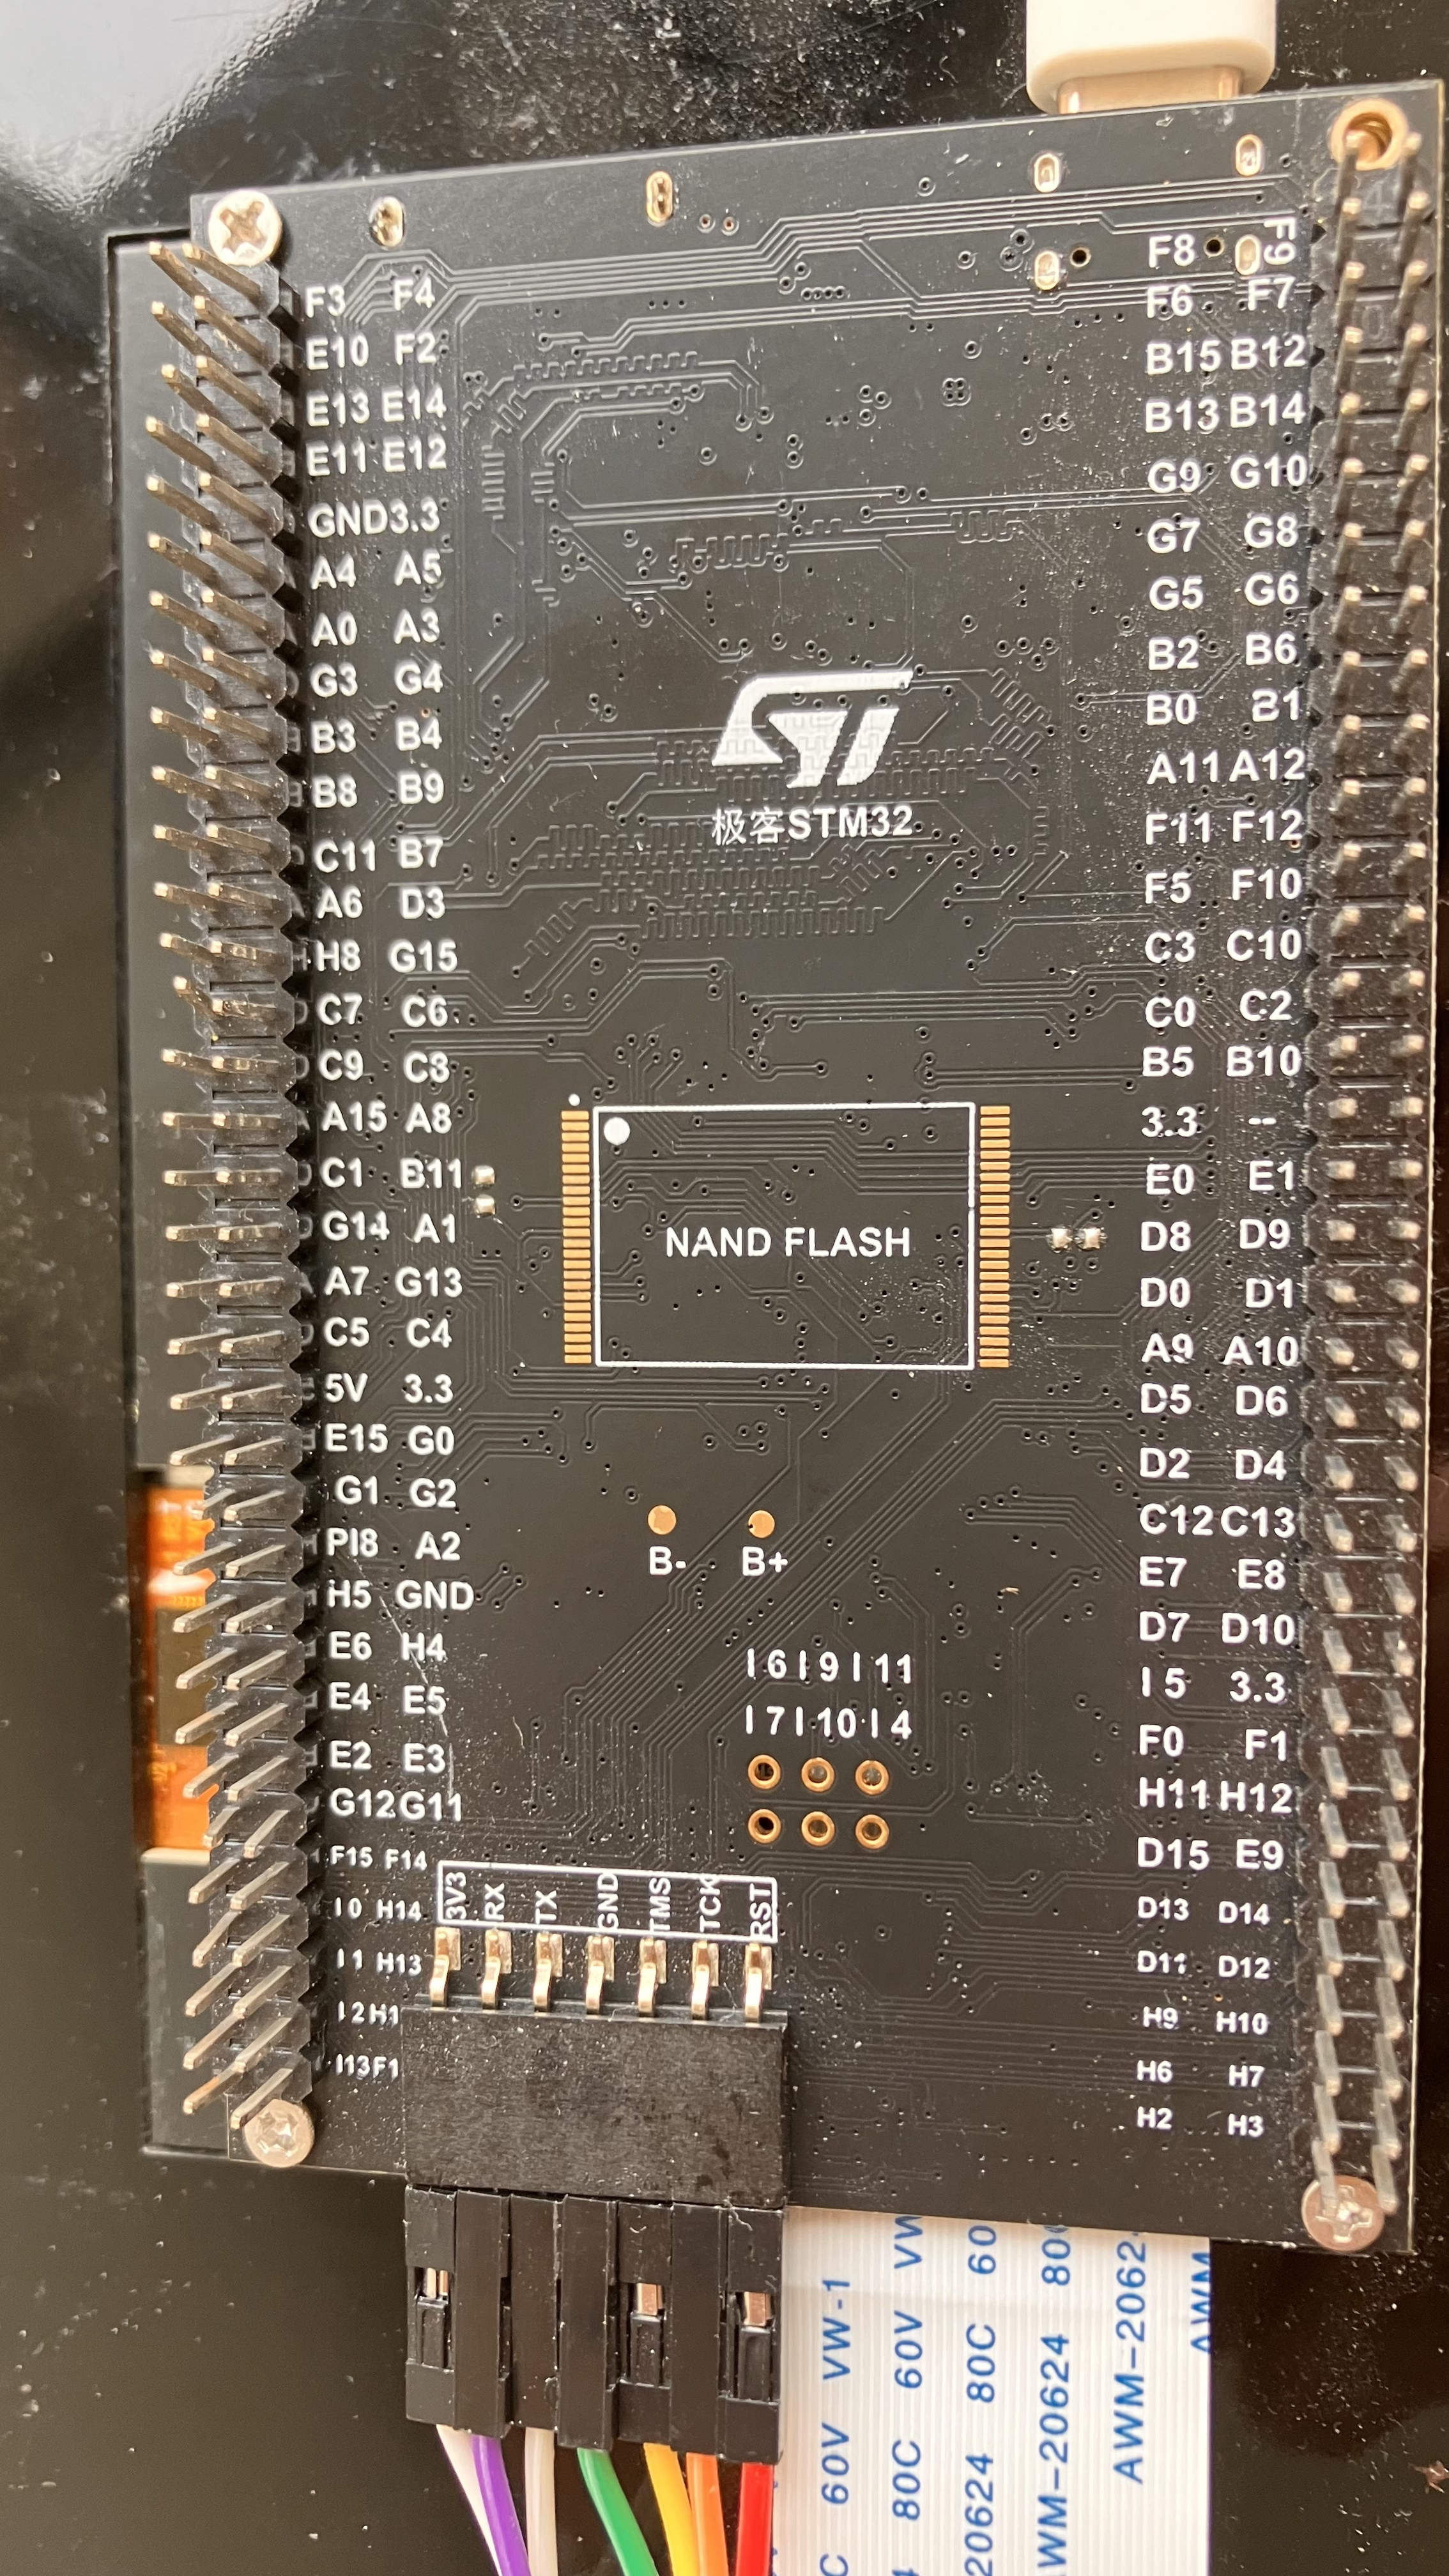
\includegraphics[width=0.66\linewidth]{../references/layout.jpg}
\caption{你的 STM32H743IIT6 核心板背面丝印。找 \texttt{B8}、\texttt{B9}、\texttt{3.3}、\texttt{GND}。}
\end{figure}

照片中可见左右两排 GPIO 丝印。优先找左侧的 \texttt{B8}、\texttt{B9} 作为 I2C1。右侧也有多个 \texttt{3.3}，左侧和底部有 \texttt{GND}。

\section{空间接线图}

\begin{center}
\begin{tikzpicture}[font=\small, node distance=10mm]
  \node[draw,rounded corners,fill=board,text=white,align=center,minimum width=48mm,minimum height=58mm] (stm) {STM32H743IIT6\\核心板};
  \node[draw,rounded corners,fill=sensor,align=center,right=42mm of stm,minimum width=35mm,minimum height=27mm] (as) {AS7343\\光谱};
  \node[draw,rounded corners,fill=sensor,align=center,below=16mm of as,minimum width=35mm,minimum height=27mm] (tsl) {TSL2591\\强度};

  \coordinate (p33) at ($(stm.east)+(0,18mm)$);
  \coordinate (pgnd) at ($(stm.east)+(0,8mm)$);
  \coordinate (pscl) at ($(stm.east)+(0,-5mm)$);
  \coordinate (psda) at ($(stm.east)+(0,-16mm)$);

  \node[left=1mm of p33,text=white] {3.3};
  \node[left=1mm of pgnd,text=white] {GND};
  \node[left=1mm of pscl,text=white] {B8/SCL};
  \node[left=1mm of psda,text=white] {B9/SDA};

  \coordinate (asv) at ($(as.west)+(0,8mm)$);
  \coordinate (asg) at ($(as.west)+(0,2mm)$);
  \coordinate (asscl) at ($(as.west)+(0,-5mm)$);
  \coordinate (assda) at ($(as.west)+(0,-12mm)$);
  \coordinate (tslv) at ($(tsl.west)+(0,8mm)$);
  \coordinate (tslg) at ($(tsl.west)+(0,2mm)$);
  \coordinate (tslscl) at ($(tsl.west)+(0,-5mm)$);
  \coordinate (tslsda) at ($(tsl.west)+(0,-12mm)$);

  \draw[-{Latex},thick,orangewire] (p33) -- ++(12mm,0) |- node[pos=0.23,above]{3.3 V} (asv);
  \draw[-{Latex},thick,orangewire] (p33) -- ++(12mm,0) |- (tslv);
  \draw[-{Latex},thick,graywire] (pgnd) -- ++(17mm,0) |- node[pos=0.22,above]{GND} (asg);
  \draw[-{Latex},thick,graywire] (pgnd) -- ++(17mm,0) |- (tslg);
  \draw[-{Latex},thick,bluewire] (pscl) -- ++(22mm,0) |- node[pos=0.20,above]{SCL} (asscl);
  \draw[-{Latex},thick,bluewire] (pscl) -- ++(22mm,0) |- (tslscl);
  \draw[-{Latex},thick,greenwire] (psda) -- ++(27mm,0) |- node[pos=0.20,below]{SDA} (assda);
  \draw[-{Latex},thick,greenwire] (psda) -- ++(27mm,0) |- (tslsda);
\end{tikzpicture}
\end{center}

\section{启动图}

当前 repo 里找到的可用启动图是：

\begin{lstlisting}
docs/assets/stm32h7-trio-display.jpg
\end{lstlisting}

我把它复制为：

\begin{lstlisting}
docs/assets/aya-lala-sasa-startup.jpg
\end{lstlisting}

固件启动时应先显示该图，再进入光谱/强度绘图界面。如果你有真正的 Aya / aya-lala-sasa 原图，把路径给我，我可以替换这个 placeholder。

\begin{figure}[h]
\centering
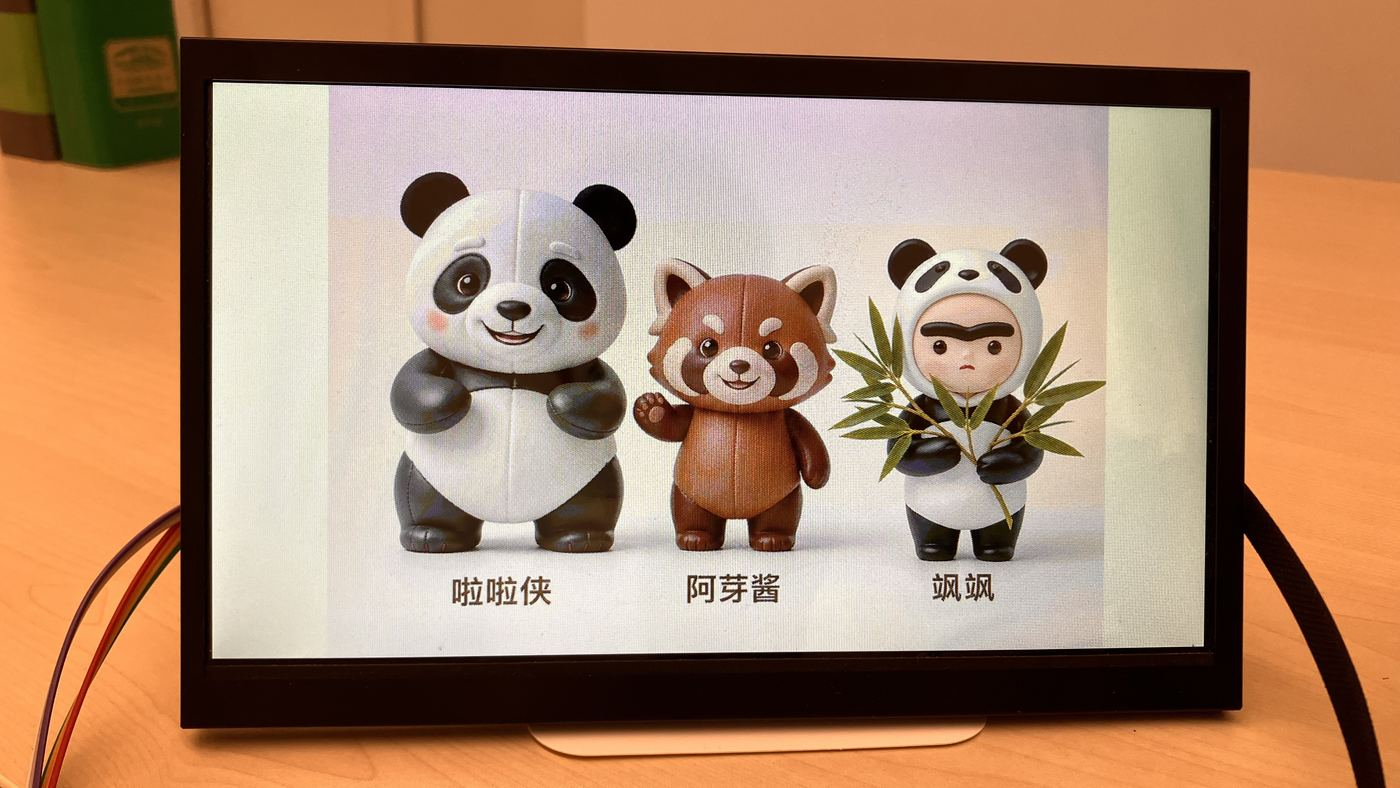
\includegraphics[width=0.42\linewidth]{../docs/assets/aya-lala-sasa-startup.jpg}
\caption{当前启动图 placeholder。}
\end{figure}

\section{采样和画图必须分离}

不要在传感器读取循环里直接画图。正确结构如下：

\begin{center}
\begin{tikzpicture}[node distance=9mm, font=\small]
  \node[draw,rounded corners,fill=blue!10,minimum width=42mm] (timer) {硬件时间戳};
  \node[draw,rounded corners,fill=green!10,below=of timer,minimum width=54mm] (acq) {高优先级 I2C 采样};
  \node[draw,rounded corners,fill=yellow!10,below=of acq,minimum width=42mm] (ring) {RAM ring buffer};
  \node[draw,rounded corners,fill=orange!10,below left=11mm and 4mm of ring,minimum width=42mm] (usb) {USB/UART 原始数据};
  \node[draw,rounded corners,fill=purple!10,below right=11mm and 4mm of ring,minimum width=42mm] (lcd) {LCD 低速绘图};
  \draw[-{Latex},thick] (timer) -- (acq);
  \draw[-{Latex},thick] (acq) -- (ring);
  \draw[-{Latex},thick] (ring) -- (usb);
  \draw[-{Latex},thick] (ring) -- (lcd);
\end{tikzpicture}
\end{center}

建议：

\begin{itemize}
  \item 采样 loop 尽可能只读传感器并写 ring buffer；
  \item LCD 刷新 10--30 Hz 即可；
  \item USB/UART 输出原始 CSV 或二进制帧；
  \item PC 端再画高质量图。
\end{itemize}

\section{输出数据格式}

PC 端脚本期望 STM32 输出：

\begin{lstlisting}
us,seq,tsl_ch0,tsl_ch1,tsl_visible,as415,as445,as480,as515,as555,as590,as630,as680,asnir,asclear
\end{lstlisting}

对应脚本：

\begin{lstlisting}
python scripts/stm32_sensor_serial_capture_plot.py --port COMx --duration 10
\end{lstlisting}

输出包含：

\begin{itemize}
  \item AS7343 最新可见光谱折线；
  \item TSL2591 intensity 随时间变化；
  \item CSV 原始数据；
  \item PNG 图。
\end{itemize}

\section{速度判断}

STM32H743 很快：官方数据手册给出 Cortex-M7 最高 480 MHz、最多 168 个 GPIO、4 个 I2C FM+ 接口、3 个 16-bit ADC 最高 3.6 MSPS，并有 LTDC/DMA2D 图形硬件。问题不是 STM32 速度，而是传感器速度。

AS7343 数据手册给出积分时间公式：

\[
t_{\mathrm{int}}=(ATIME+1)(ASTEP+1)2.78\,\mu s
\]

TSL2591 常规 ALS 积分时间最低约 100 ms。因此：

\begin{itemize}
  \item TSL2591 可以验证慢速总强度，不适合验证真正 100 ms 以下波形；
  \item AS7343 可以做较快谱指纹，但完整多通道光谱帧仍受积分和读出限制；
  \item 若要验证 100 ms 或更快的 merged intensity，建议光电二极管 + 跨阻放大器 + STM32 ADC/DMA；
  \item 若要生产中高速调光，使用开环 LUT，不必实时测量。
\end{itemize}

\section{下一步}

请确认 Windows 能看到 ST-Link 或 USB 串口。正常情况下应该出现：

\begin{itemize}
  \item ST-Link USB device；
  \item 或一个新的 \texttt{COMx}；
  \item OpenOCD 不再报 \texttt{open failed}。
\end{itemize}

然后才能 flash STM32，并真正读取 AS7343/TSL2591。

\section{资料来源}

\begin{itemize}
  \item STMicroelectronics, STM32H742xI/G STM32H743xI/G datasheet, DS12110 Rev. 11, January 2026. \url{https://www.st.com/resource/en/datasheet/stm32h743vi.pdf}
  \item ams OSRAM, AS7343 14-Channel Multi-Spectral Sensor datasheet, DS001046 v6-00, 2023. \url{https://look.ams-osram.com/m/5f2d27fff9a874d2/original/AS7343-14-Channel-Multi-Spectral-Sensor.pdf}
  \item ams OSRAM, TSL2591 Light-to-Digital Converter datasheet, DS000338 v3-00, 2023. \url{https://look.ams-osram.com/m/c901de8e97608f8/original/TSL2591-DS000338.pdf}
\end{itemize}

\end{document}
